\documentclass[10pt]{article}
\usepackage[margin=0.7in]{geometry}
\usepackage[T1]{fontenc}
\usepackage{lmodern}
\usepackage{graphicx,booktabs,tabularx}
\usepackage[hidelinks]{hyperref}
\setlength{\parindent}{0pt}
\setlength{\parskip}{5pt}
\newcommand{\repo}{https://github.com/aburan28/crypto/blob/codex/envoy-fpga-crypto-pq-20261017/integrations/envoy-fpga-crypto/}
\begin{document}
\begin{center}
{\Large Envoy RTL: Ubuntu CI compatibility}\\[3pt]
2026-10-18 \quad Run batch: \texttt{envoy-fpga-20261018-ci-compat}
\end{center}

The PR's module jobs passed core tests, then failed RTL lint under Ubuntu's
Verilator 5.020. Earlier local validation used 5.032. The unchanged parent
reproduces seven array-loop errors and four fatal width warnings with 5.020.
The fix raises the static loop-unrolling limit to 256 and explicitly
zero-extends each 23-bit NTT multiplier operand to 32 bits. Fatal
\texttt{-Wall}, assertions, test cases and structural checks remain enabled.

\begin{center}
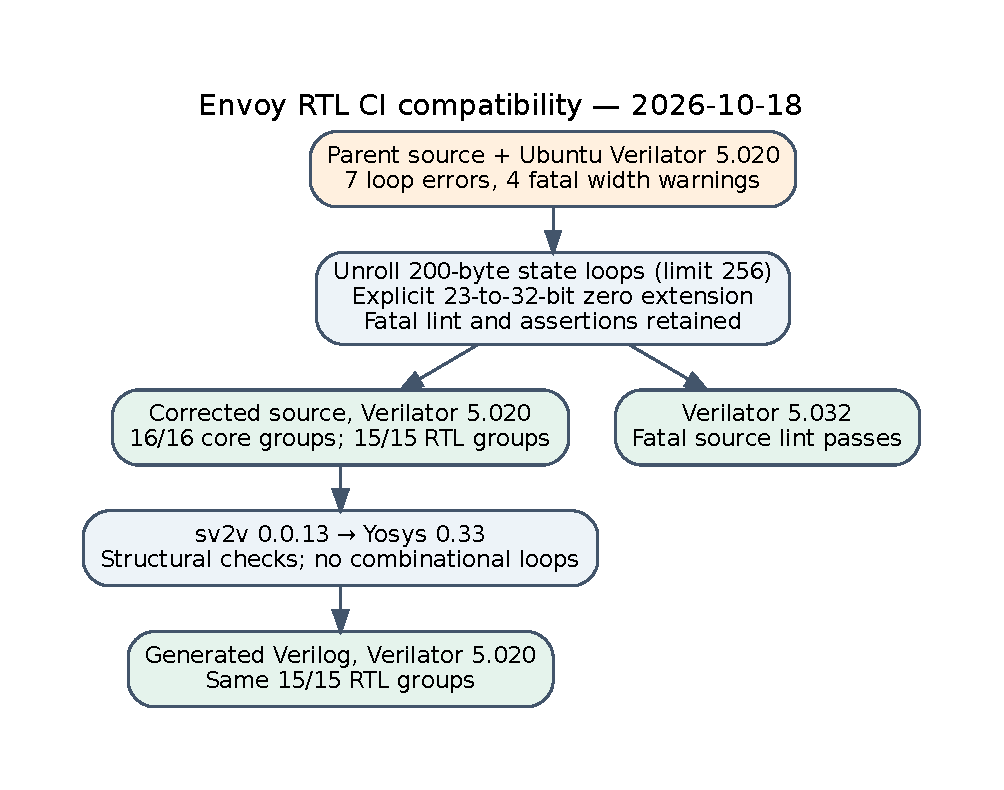
\includegraphics[width=0.94\textwidth,height=0.38\textheight,keepaspectratio]{flow.pdf}
\end{center}
\textbf{Figure 1.} Validation stages, not performance measurements.
The synthesis result repeats the same test groups; it is not a formal
equivalence proof or 30 independent specifications. Source: \texttt{flow.dot}.

\begin{tabularx}{\textwidth}{@{}lX@{}}
\toprule
Check & Observed result \\
\midrule
Core transport & 16/16 groups passed. \\
Source RTL, 5.020 & Fatal lint passed; 15/15 groups passed. \\
Yosys 0.33 replay & Structural checks passed; same 15/15 groups passed. \\
Source lint, 5.032 & Passed; full simulation was not repeated with this version. \\
Scoped workflow & actionlint 1.7.7 passed. \\
Root Rust gate & Exit 101 before tests: same 26 errors in unchanged source. \\
\bottomrule
\end{tabularx}

\textbf{Environment and limits.} Debian 13, GCC 14.2.0, OpenSSL 3.5.7;
Ubuntu packages Verilator 5.020 and Yosys 0.33; sv2v 0.0.13. The RTL tool
versions match CI, but the full hosted runner environment does not.
Fixtures and independent oracles are unchanged; seed
\texttt{0x4650433252544c}. No optional liboqs/BoringSSL/live-Envoy suite,
physical FPGA test or cryptographic timing measurement was run.

\textbf{Retained failures and gates.} Both failing module CI logs, the local
reproduction, an unroll-only attempt, package-relocation failures and an
actionlint working-directory error are retained locally. Existing workflow duplicate
keys, curve-registry/name failures and root Rust errors remain outside this
change. No submitted reviews or inline threads were present in the initial
snapshot; neutral Cursor checks reported usage limits. New-head CI and actual
review requirements must still be satisfied before merging.

\textbf{Provenance.} Extends parent
\texttt{e6369b99328ab2b6ee301679c133691000c1f31a},
\href{https://github.com/aburan28/crypto/pull/2122}{PR \#2122}.
The \href{\repo docs/receipts/2026-10-18-ci-compat/README.md}{summary receipt}
records source hashes and aggregate outcomes. The new local raw archive and
frozen run manifest await upload approval; their hashes identify the
execution-era snapshot. The
\href{\repo docs/reports/2026-10-18-ci-compat/README.md}{full report}
records scope and reproduction. Older evidence remains unchanged.
Complete crypto controllers, entropy/key custody, FPC1/F2/AFI integration,
physical and side-channel validation, and measured acceleration remain open.
\end{document}
